%%% $Id: PSDC-940-005.tex,v 1.9 2011/04/18 23:17:36 schastel Exp $
\documentclass[panstarrs,spec]{panstarrs}
\usepackage{nonfloat}
\usepackage{caption}

\usepackage{etoolbox}
\patchcmd{\thebibliography}{\chapter*}{\subsection*}{}{}

\newcommand{\outformatversion}{%
  \texttt{PS1\_DV3}}

\newcommand{\commentFrom}[4]{%
  \mbox{ }\\\null\hfill\begin{tabular}{|p{4in}}
    \hline
    \emph{Comment from {#1} (#2)}: {#3}\\
    \hline
    Answer: {#4}\\
    \hline
  \end{tabular}}

\newcommand{\commentFromSC}[3]{%
  \commentFrom{SC}{#1}{#2}{#3}}

% basic document variables
\title{IPP-MOPS ICD}
\subtitle{Pan-STARRS IPP-MOPS ICD for PS-1}
\shorttitle{IPP-MOPS ICD}
\author{\parbox{3in}{Serge Chastel; Larry Denneau, Jr.; Denver Green; Robert Jedicke; Eugene Magnier}}
\audience{Pan-STARRS PMO}
\group{Pan-STARRS IPP \& MOPS}
\project{Pan-STARRS PS-1}
\organization{Institute for Astronomy}
\version{03}
\docnumber{PSDC-940-005}

\begin{document}
\maketitle
\sloppy

\RevisionsStart
% version  Date            Description
04 & 2012 Nov 20  & Modifications integrating DG comments/questions \\ 
\hline
03 & 2012 Oct 04  & \texttt{PS1\_DV3}: Fitted trails, new parameters\\ 
\hline
02 & 2011 Apr 19  & Synchronization with "ICD Lite" wiki page \\ 
\hline
01 & 2010 Oct 27  & New CMF Parameters \\ 
\hline
00 & 2006 Mar 01  & Initial version \\ 
\hline
\RevisionsEnd

%%%%%%%%%%%%%%%%%%%%%%%%%%%%%%%%%%%%%%%%%%%%%%%%%%%%%%%%%%%%%%%%%%%%%%%%% 

\bibliographystyle{amsplain}
\bibliography{icd}

\DocumentsInternal
PSDC-230-001 & PS-1 Design Reference Mission \\ \hline
PSDC-430-011 & Pan-STARRS PS-1 IPP System/Subsystem Design Description \\ \hline
PSDC-510-001 & Pan-STARRS PS-1 MOPS System Concept Definition \\ \hline
PSDC-530-003 & Pan-STARRS PS-1 MOPS Software Design Description \\ \hline
\DocumentsExternal
\DocumentsEnd

\tableofcontents
\pagebreak 
\pagenumbering{arabic}

%%%%%%%%%%%%%%%%%%%%%%%%%%%%%%%%%%%%%%%%%%%%%%%%%%%%%%%%%%%%%%%%%%%%%%%%% 

\section{Scope}

\subsection{Identification}

This document defines the interface between the Image Processing
Pipeline (IPP) and Moving Object Processing System (MOPS) for the
Panoramic Survey Telescope and Rapid Response System (Pan-STARRS)
for the prototype telescope PS-1, and is a System-level controlled
specification/design description document in the official Pan-STARRS
engineering specification tree.

\subsection{System Overview}

The Institute for Astronomy at the University of Hawai`i is developing
a large optical synoptic survey telescope system, the Panoramic Survey
Telescope and Rapid Response System (Pan-STARRS). The science goals,
priorities, top-level concept of operations with associated
operational requirements, and system performance drivers with
associated system performance requirements are described in the
Pan-STARRS Science Goals Statement (SGS).  As described in this
document, The system conceptual design for Pan-STARRS utilizes an
array of four 1.8m telescopes each with a 7 degree$^2$ field of view,
giving the system an \'etendue larger than all existing survey
instruments combined (defined as the product of the collecting area
$A$ multiplied by the field-of-view solid angle $\Omega$).  Each
telescope will be equipped with a 1 billion pixel CCD camera with low
noise and rapid read-out, and the data will be reduced in near real
time to produce both cumulative static sky and difference images from
which transient, moving, and variable objects can be
detected. Pan-STARRS will be able to survey up to $\approx 6,000$
degree$^{2}$ per night to a detection limit of approximately 24$^{th}$
magnitude.  This unique combination of sensitivity and sky coverage
will open up many new possibilities in time domain astronomy including
a major goal of surveying the Potentially Hazardous Object (PHO)
population down to a diameter of $\approx 300$ meters.  In addition,
the Pan-STARRS data will be used to investigate a broad range of
astronomical problems of extreme current interest concerning the Solar
System, the Galaxy, and the Cosmos at large.  A prototype single
telescope system, PS-1, is being developed as a preliminary step
before construction of the complete four telescope system.

\begin{tabular}{ll}
  Project sponsor:&	AFRL, United States Air Force \\
  Acquirer:       &	University of Hawaii Institute for Astronomy \\
  User: 	  &	Astronomical community \\
  Developer:      &	University of Hawaii Institute for Astronomy, participating \\
  &       institutions, and associated subcontractors	
\end{tabular}

\subsection{Document Overview}

This document identifies the interface between the IPP and MOPS
subsystems of the Pan-STARRS PS-1 Telescope.

%%%%%%%%%%%%%%%%%%%%%%%%%%%%%%%%%%%%%%%%%%%%%%%%%%%%%%%%%%%%%%%%%%%%%%%%% 

\DocumentsInternalSection
PSDC-230-001  &   PS-1 Design Reference Mission \\ \hline
PSDC-230-002  &   PS-1 System Concept Definition \\ \hline
\DocumentsExternalSection
POSIX Standard & Open Group Based Specifications Issue 6, IEEE Std 1003.1, 2003 \\
FITS Standard & Definition of the Flexible Image Transport System (FITS),
March 29, 1999, NOST 100-2.0 \\
\DocumentsEnd

\subsection{Acronyms}

\begin{table}
  \small
  \caption{Acronyms used in this document\label{table-acronyms}}
  \begin{tabular}{ll}
    \hline
    {\bf Acronym}            & {\bf Definition} \\
    \hline
    ADU & Analog to Digital Units (counts in an image) \\
    ICRS  & International Celestial Reference System \\
    IPP   & Pan-STARRS Image Processing Pipeline \\
    FPA   & Focal Plane Array \\
    MOPS  & Pan-STARRS Moving Object Processing System \\
    MPC   & Center for Astrophysics Minor Planet Center \\
    TTI   & Transient-Time Interval (about 60 minutes) \\
    \hline
  \end{tabular}
\end{table}

\section{Interface Overview}

\subsection{Pan-STARRS Software Interfaces}

The Pan-STARRS PS-1 Telescope system has multiple
subsystem-to-subsystem interfaces, illustrated in
Figure~\ref{fig:overview}.  The subsystem-to-subsystem interfaces are
each documented in separate documents.  The interface numbers refer to
the Pan-STARRS Document Control numbering scheme for the interface
documents.  All Interface Control Documents are numbered
PSDC-940-XXX-VV, while all Interface Requirements Specifications are
numbered PSDC-930-XXX-VV, where XXX is the number listed above and VV
is a document version number.  Table~\ref{tab:overview} lists the
organizational structure of all Pan-STARRS interfaces, giving the
corresponding interface number listed in Figure~\ref{fig:overview},
the group of data being transferred (the assembly), the method in
which the data is formatted (packing), and the data transfer method
(protocol).

\begin{figure}
  \begin{center}
    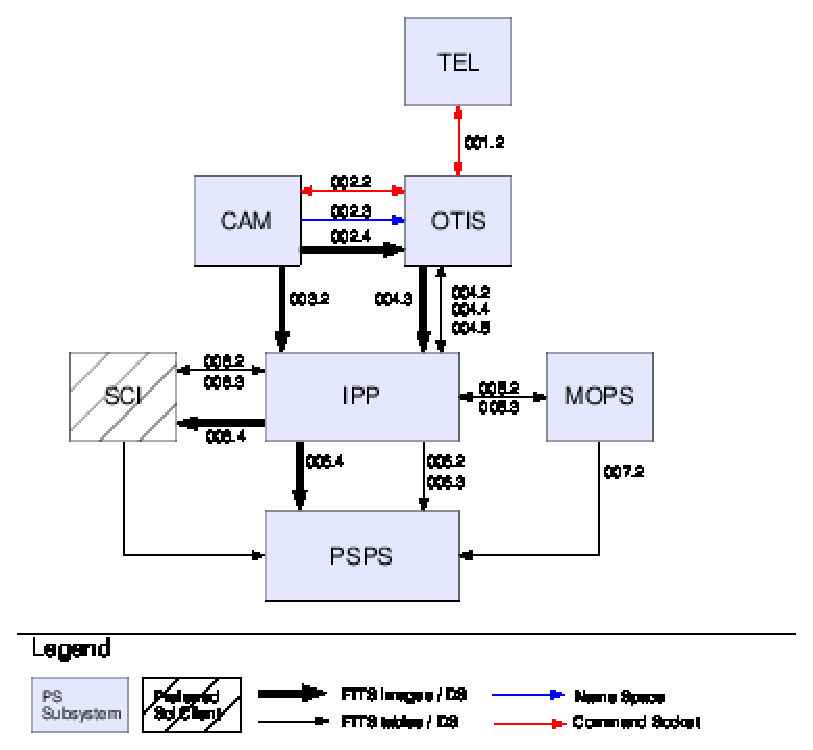
\epsfig{file=figures/PSSWIF.eps}
    \caption{Overview of Pan-STARRS Software Interfaces.}
    \label{fig:overview}
  \end{center}
\end{figure}

This document discusses the software interface between IPP and MOPS.
IPP must send transient detection descriptions to the MOPS; MOPS must
be able to query the IPP regarding whether a particular (RA, Dec) pair
could have been detected in a particular focal plane array (FPA).
This document defines the data to be transferred between IPP and MOPS
and the mechanisms to be used for that interchange.  These interfaces
are identified as \#005 in Figure~\ref{fig:overview}.  The Interfaces
addressed by this document are marked in the table.

\begin{table}
  \begin{center}
    \caption{Pan-STARRS Interface Data Organization}
    \label{tab:overview}
    \begin{tabular}{|l|l|l|l|}
      \hline
      {\bf Interface \#} & {\bf Assembly} & {\bf Packaging} & {\bf Protocol} \\ \hline
      001.2 & Telescope Commands     & EOST Command Language      & Command Socket \\
      002.2 & Camera Commands        & Conductor Command Language & Command Socket \\
      002.3 & Camera Status          & ???                        & Shared Name Space \\
      002.4 & IQ Images              & FITS Images                & Data Store \\
      003.2 & GPC Images \& Metadata & FITS Images \& Headers     & Data Store \\
      \hline
      004.2 & OTIS Metadata          & FITS Tables                & Data Store \\
      004.3 & ISP Images \& Metadata & FITS Images \& Headers     & Data Store \\
      004.4 & Reference Star Catalog & FITS Tables                & Data Store \\
      004.5 & Focal Plane Layout     & FITS Tables                & Data Store \\
      \hline
      005.2 & Detections             & FITS Tables                & Data Store \\
      005.3 & Test Positions         & FITS Tables                & Data Store \\
      006.2 & Detections             & FITS Tables                & Data Store \\
      006.3 & Metadata               & FITS Tables                & Data Store \\
      006.4 & Images                 & FITS Tables                & Data Store \\
      007.2 & Orbits \& Detections   & FITS Tables                & Data Store \\
      008.2 & Detections             & FITS Tables                & Data Store \\
      008.3 & Metadata               & FITS Tables                & Data Store \\
      008.4 & Images                 & FITS Tables                & Data Store \\
      \hline
    \end{tabular}
  \end{center}
\end{table}

Layers of network communications are often classified using the
\htmladdnormallink{OSI Reference
  Model}{http://en.wikipedia.org/wiki/OSI_reference_model}.  When addressing
network connectivity between subsystem interfaces, this
Interface Control Document is primarily concerned with two highest
layers of the interface communication: the presentation layer, or how
the data is packaged, and the application layer, or the high-level details of the
data contents.  The lower layers of the network communication in the OSI model
are addressed briefly below.

The leased line between the IPP and MOPS is currently expected to have a practical
maximum sustainable throughput of 50Mbits/s, since the systems will be connected
through the University of Hawaii ITS network.  Higher and lower bit rates are available,
and the cost diffferences are quite significant.

\subsubsection{Physical Layer}

MOPS and IPP will each be connected to local inbound and outbound hardware
interfaces at rates of no less than 1Gbit/sec using fiber or twisted pair
and onboard NICs where possible.

\subsubsection{Data Link Layer}

The endpoints of the route between IPP and MOPS will be Gigabit
Ethernet with normal (1500 byte) max. transmission units (MTU).

\subsubsection{Network Layer}

Internet Protocol v4 will be used.  Data Store's HTTP
server will have an IP address visible (routable) to IPP.

\subsubsection{Transport Layer}

TCP will be used on top of IPv4.

\subsubsection{Session Layer}

IPP-MOPS communication will take place entirely via the Data Store
mechanism.

\subsubsection{Presentation Layer}

All data exchanged between IPP and MOPS will be in the form of FITS
Tables and FITS images.

The primary header will not contain any information beyond that
written automatically by cfitsio, and is present only for compliance
with the FITS standard.

Though efforts have been made to avoid this from occurring, where
header keyword names are longer than the usual 8 character maximum,
the HIERARCH convention will be used (see the NASA webpages:
\htmladdnormallink{Registered FITS
  Convention}{http://fits.gsfc.nasa.gov/registry/hierarch_keyword.html}
and \htmladdnormallink{4.12.4 HIERARCH Convention for Extended Keyword
  Names}{http://heasarc.nasa.gov/docs/software/fitsio/c/f_user/node28.html}).

\subsection{IPP-MOPS Exchange}

MOPS requires from the IPP a stream of transient detections and their
FPA metadata obtained from processing of difference images acquired by
the PS-1 camera. 

IPP is additionally required by MOPS to be able to indicate whether a
set of detections (with RA, Dec, flux, length, orientation, etc.) on a
previously acquired FPA was detectable by the PS-1 telescope. This
functionality is provided through the detectability server.

\subsubsection{Conventions}

\begin{enumerate}
\item Celestial coordinates are in ICRS;
\item Magnitudes are AB magnitudes (flux zero point is 3631 Jy);
\item Unless otherwise noted, error values are statistical only, and
  include no contribution by systematic errors.
\end{enumerate}

\subsubsection{Transient Detection and Metadata Exchange}

Transient detections and their metadata are assembled nightly into
FITS files, one file per FPA.  IPP will submit outgoing data into the
IPP-MOPS outbound datastore.  Metadata for the detections belonging to
a FPA will be described in the file's FITS headers, and detection data
will be listed in a subsequent FITS BINTABLE table in the same file.

Each column in the FITS table shall correspond to a detection attribute.
The data type of a FITS column shall be chosen to represent the attribute
without loss of information.

The FITS table will include all detections within an exposure.

Duplicates from overlapping skycells will have been filtered out by
IPP, with the measurements from the source closest to the centre of a
skycell included (and all others discarded).

\subsubsection{Detectability}

MOPS will need to query the IPP periodically to inquire whether a
particular elongated trailed detection specified by a ($RA_0$,
$Dec_0$, $Time_0$, $RA_1$, $Dec_1$, $Time_1$) tuple was detectable by
the PS-1 telescope.  This query is important in evaluating
``non-detections,'' or failures of MOPS to locate predicted detections
of a known object, and for accurate simulation of detections of
synthetic objects that are injected into the MOPS pipeline to measure
efficiency.

MOPS will assemble a list of (RA, Dec, Time) tuples in a single FITS
file and submit them to the MOPS-IPP outgoing datastore.  Later MOPS
will poll the IPP datastore for results of this query.  If results of
a query do not appear after a pre-configured timeout, an operator is
notified.

\subsubsection{Table Description Files}

FITS tables generated by IPP or MOPS shall be described by table
description files.  These files shall be controlled by CVS, with the
authoritative versions of these files being the ones contained in
Appendix A of this document. FITS header data units (HDUs) which do
not conform to the corresponding table description files shall be
rejected by the receiver, and the ingest software shall notify an
operator about the error.

In addition to the required keywords specified in the FITS standard
for a BINTABLE extension, each FITS HDU shall have the following
keywords:

\begin{itemize}
\item{EXTNAME} - A \emph{string} giving a unique name for the metadata
  table. Such a name shall contain only the characters a-z, A-Z, and
  ``\_''.
\item{CMFVERSION} - A \emph{string} specifying the version of the
  table description file for this table.
\end{itemize}

The format of the metadata tables is described in the following sections.

\subsubsection{Fields in Table Description Files}

The IPP software generating the FITS tables may change. Parameters,
i.e. columns in FITS tables, may also be added requiring changes both
in ICD and in software. To keep track of such changes, a Version will
be assigned to each keyword in the tables descriptions.

To improve the readability, keywords appearing only in the
\outformatversion{} software version are shown. For previous releases
of this documentation and learn about the former output format,
checkout \htmladdnormallink{the older SVN revision
  34506}{https://svn.pan-starrs.ifa.hawaii.edu/repo/ipp/trunk/ppTranslate/documentation/ICD}.

The following conventions for the Version numbering is used: $X+$
(where $X$ is the output format version in \texttt{PS1\_DV$X$}) means
that the keyword appeared in software version X until the current
version.

\subsubsection{ICD/Software Versions}

\begin{tabular}{|c|c|c|c|p{3in}|}
  \hline
  SW Version & ICD Version & Output Version & Software Tag & Comment \\
  \hline
  0 & 00 & 0 & n/a & Preliminary ICD. No sw tag \\
  1 & 01 & \texttt{PS1\_DV1} & 20100823 & First software release \\
  2 & 01 & \texttt{PS1\_DV2} & 20101029 & "V2" software version \\
  2 & 02 & \texttt{PS1\_DV2} & 20110406 & Deletion of "ICD lite" wiki page (Documentation update only)\\
  4 & 03 & \texttt{PS1\_DV3} & \emph{No tag yet} &  Extended parameters (fitted trails), warp-stack\\
  \hline
\end{tabular}

\subsubsection{Transfer via Data Store}

The FITS files containing metadata shall be tranferred using the protocol 
described in [Data Store doc]. There will be one instance of a datastore 
within IPP that will be used to submit transient detections and results 
of detectability queries to MOPS, and
another instance residing within MOPS to submit detectability requests to the IPP.

During a datastore transaction, the ``sender'' places a file into the datastore with a unique
transfer ID. The ``receiver'' must regularly poll the datastore to
detect new FITS files. The receiver then downloads each file from a URL
provided by the Data Store interface. The receiver is responsible for
managing which files it has already downloaded. Files remain in
the datastore for a preset period of time and then are deleted without
warning. If a file transfer fails, the receiver may retry the transfer,
If a retry fails, the failure must be resolved by operator intervention.

The data transfers will have the following parameters:

\begin{table}[htbp]
  \begin{center}
    \caption{Data transfer parameters}
    \begin{tabular}{|l|l|l|}
      \hline
      \hline
      {\bf Parameter} & {\bf IPP to MOPS} & {\bf MOPS to IPP} \\ 
      \hline
      Dump interval & Per FPA & Per FPA \\
      Max polling Interval & 60s & 60s \\
      File Lifetime & 30 days & 10 days \\
      Datastore location & IPP & MOPS \\ \hline
    \end{tabular}
  \end{center}
\end{table}

\subsection{Transient Detection List}

IPP will submit all transient detections per FPA and their associated
metadata in a single FITS file.  The metadata will be placed in FITS
header data unit (HDU) key-value pairs, and the detection attributes
will be placed in the associated FITS table following the header.  All
time-dependent table values shall be provided at the midpoint of the
exposure.

{\centering%
  \tabcaption{IPP-MOPS Data Types Definition\label{table-datatypes}}
  \begin{longtable}{|cp{5in}|}
    \hline
    \textbf{Alias} & \textbf{Description} \\
    \texttt{bool} & (Not a FITS type) An enumerated type defining a Boolean
    value, either \texttt{true} or \texttt{false}\\
    \texttt{char($n$)} & (Not a FITS type) A sequence of exactly $n$ bytes that
    can be interpreted
    as a sequence of ASCII characters\\
    \texttt{HH:MM:SS.sss} & (Not a FITS type) a \texttt{char(12)} encoding
    a time or an angle: (1) the hours \texttt{HH} are encoded with two
    decimal figures; (2) a separator \texttt{:} between the hours and
    the minutes; (3) the minutes \texttt{MM} are encoded with two
    decimal figures; (4) a separator \texttt{:} between the minutes
    and the seconds; (5) the seconds \texttt{SS} are encoded with two
    decimal figures; (6) a separator \texttt{.} between the seconds
    and the milli(arc)seconds; (7)
    the milli(arc)seconds \texttt{ss} are encoded with three decimal figures; \\
    \texttt{sDD:MM:SS} & (Not a FITS type) a \texttt{char(9)} encoding an
    angle. (1) \texttt{s} is either the \texttt{+} or \texttt{-} sign;
    (2) \texttt{DD} is the number of degrees encoded with two decimal
    figures; (3) a separator \texttt{:} between the degrees and the
    minutes; (4) the minutes \texttt{MM} are encoded with two decimal
    figures; (5) a separator \texttt{:} between the minutes and the
    seconds; (6) the
    seconds \texttt{SS} are encoded with two decimal figures;\\
    \texttt{enum} & (Not a FITS type) a \texttt{string} having a fixed number of
    different values. The explicit set of values shall be expressed in
    this ICD.\\
    \texttt{F32} & (FITS type) IEEE 32-bit single precision floating point real numbers \\
    \texttt{F64} & (FITS type) IEEE 64-bit double precision floating point real numbers \\
    \texttt{S16} & (FITS type) 16-bit signed integer \\
    \texttt{S32} & (FITS type) 32-bit signed integer \\
    \texttt{S64} & (FITS type) 64-bit signed integer \\
    \texttt{string} & (Not a FITS type) Sequence of bytes of arbitrary length 
    usually interpreted as a sequence of ASCII characters \\
    \texttt{U16} & (FITS type) 16-bit unsigned integer \\
    \texttt{U32} & (FITS type) 32-bit unsigned integer \\
    \hline
  \end{longtable}
}

In addition to the required BINTABLE extension header keywords
described above (TODO: Where? What?), the FITS header shall include the
keywords shown in tables relative to versioning
\ref{table-keywords-versioning}, data provenance
\ref{table-keywords-provenance}, and exposure
\ref{table-keywords-exposure}. The subsequent FITS table, with EXTNAME
of \code{MOPS_TRANSIENT_DETECTIONS}, shall include columns whose
definitions are listed in table \ref{table-detections} and, when trail
fitting has been succesfully performed, \ref{table-detections-ext}.

\begin{center}
  \begin{longtable}{|lcp{0.5in}p{3in}|}
    \caption{IPP-MOPS Transient Detection Keywords:\\ Version Information}\label{table-keywords-versioning}\\
    \hline\hline
    \multicolumn{4}{|l|}{\null\hspace*{1in}\textbf{Version Information}}\\
    \hline\hline
    {\bf FITS Keyword}
    & \parbox{0.5in}{\textbf{Version}}
    & {\bf Precision}
    & {\bf Description} \\
    \hline
    SWSOURCE & 1+ & \texttt{string} & source of software (e.g., "60eb6cdc-a59c-4636-a4e0-dba66a9721fd") \\
    \hline
    SWVERSN & 1+ & \texttt{string} & version of software (e.g., "trunk/ppMops@24658") \\
    \hline
    HIERARCH CMFVERSION & 2+ & \texttt{enum} & \texttt{PS1\_DV3} \\
    \hline\hline
  \end{longtable}
\end{center}

\begin{center}
  \begin{longtable}{|lcp{0.5in}p{3in}|}
    \caption{IPP-MOPS Transient Detection Keywords:\\ Provenance Information}\label{table-keywords-provenance}\\
    \hline\hline
    \multicolumn{4}{|l|}{\null\hspace{10mm}\textbf{Provenance Information}}\\
    \hline \hline
    {\bf FITS Keyword}
    & \parbox{0.5in}{\textbf{Version}}
    & {\bf Precision}
    & {\bf Description} \\
    \hline
    EXP\_NAME & 1+ & \texttt{string} & Exposure name (e.g., "o1234g5678")\\
    \hline
    EXP\_ID & 1+ & \texttt{S64} & Exposure identifier \\
    \hline
    CHIP\_ID & 1+ & \texttt{S64} & Chip stage identifier \\
    \hline
    CAM\_ID & 1+ & \texttt{S64} & Camera stage identifier \\
    \hline
    FAKE\_ID & 1+ & \texttt{S64} & Fake stage identifier \\
    \hline
    WARP\_ID  & 1+ & \texttt{S64} & Warp stage identifier \\
    \hline
    DIFF\_ID & 1+ & \texttt{S64} & Diff stage \\
    \hline
    DIFF\_POS & 1+ & \texttt{bool} & Sense of subtraction; \texttt{true} for forward, 
    \texttt{false} for backward\\
    \hline
  \end{longtable}
\end{center}
  
\begin{center}
  \begin{longtable}{|lcp{0.5in}p{3in}c|}
    \caption{IPP-MOPS Transient Detection Keywords:\\ Exposure Details}\label{table-keywords-exposure}\\
    \hline \hline
    \multicolumn{5}{|l|}{\null\hspace{10mm}\textbf{Exposure Details}}\\
    \hline \hline {\bf FITS Keyword}
    & \parbox{0.5in}{\textbf{Version}} & {\bf Precision} & {\bf
      Description}
    & \textbf{Units}\\
    \hline MJD-OBS & 0+ & \texttt{F64} & midpoint time of the exposure
    as a MJD and day fraction
    & N/A\\
    \hline RA & 0+ & {\tiny \texttt{HH:MM:SS.SSS}}
    & Field center RA at exposure midpoint & N/A \\
    \hline DEC & 0+ & {\tiny \texttt{sDD:MM:SS}} &
    (s is + or -) Field center declination at exposure midpoint & N/A \\
    \hline EXPTIME & 0+ & \texttt{F64}
    & Exposure time & seconds \\
    \hline ROTANGLE & 0+ & \texttt{F64}
    & Image rotation of the y-axis from local N toward E & degrees \\
    \hline FILTER & 0+ & \texttt{char(7)} & Effective filter used for
    the exposure, one of \texttt{g}, \texttt{r}, \texttt{i},
    \texttt{z}, \texttt{y}, \texttt{B},
    \texttt{V}, \texttt{w} appended with '.00000' & N/A \\
    \hline AIRMASS & 0+ & \texttt{F64}
    & Airmass at exposure midpoint & N/A\\
    \hline OBSCODE & 0+ & char(5) &
    MPC 3-character observatory code (F51 for PS1) & N/A \\
    \hline TEL\_ALT & 0+ & \texttt{F64} &
    Telescope altitude at exposure midpoint & degrees \\
    \hline TEL\_AZ & 0+ & \texttt{F64}
    & Telescope azimuth at exposure midpoint & degrees \\
    \hline SEEING & 1+ & \texttt{F32} &
    Measured seeing at diff stage & arcsec \\
    \hline MAGZP & 1+ & \texttt{F32} &
    Magnitude zero point & N/A \\
    \hline MAGZPERR & 1+ & \texttt{F32} &
    Error in magnitude zero point & N/A \\
    \hline ASTRORMS & 1+ & \texttt{F32} &
    RMS of astrometric fit & arcsec \\
    \hline CMMTOBS & 3+ & \texttt{string} &
    Comment associated to the exposure & N/A\\
    \hline OBS\_MODE & 3+ & \texttt{enum} & Observation modes list:
    3PI, CNP, ESS, M31, MD, MSS, OSS, PI, STD (Note: The exposures
    having the following PS1 observation modes are not used by MOPS:
    CAL, PR201108, SAS2, SS, STS, STS2A, STS2B) & N/A\\
    \hline DIFFTYPE & 3+ & \texttt{enum} &
    Difference type: \texttt{WW} (Warp-Warp Difference), \texttt{WS} (Warp-Stack Difference) & N/A\\
    \hline SKY & 3+ & \texttt{F64} &
    Exposure average sky background & counts/pixel \\
    \hline SHUTOUTC & 3+ & \texttt{string} &
    Camera exposure shutter open (UTC) & N/A \\
    \hline \hline
  \end{longtable}
\end{center}

\begin{center}
  \begin{longtable}{|lclp{3.5in}c|}
    \caption{IPP-MOPS Transient Detection Table Columns:\\ Detection Details}\label{table-detections}\\
    \hline \hline
    \multicolumn{5}{|l|}{\null\hspace{10mm}\textbf{Detection Details}}\\
    \hline \hline
    {\bf Column} & \textbf{Version} & {\bf Precision} & {\bf Description} & \textbf{Units}\\
    \hline
    RA & 1+ & F64 & Detection center coordinates & degrees\\
    \hline
    RA\_ERR & 1+ & F64 & Error in the detection center & degrees \\
    \hline
    DEC & 1+ & F64 & Detection center coordinates & degrees \\
    \hline
    DEC\_ERR & 1+ & F64 & Error in the detection center & degrees \\
    \hline
    MAG & 1+ & F32 & Filter magnitude & N/A \\
    \hline
    MAG\_ERR & 1+ & F32 & Filter magnitude error & N/A  \\
    \hline
    PSF\_CHI2 & 1+ & F32 & $\chi^2$ of PSF fit & N/A \\
    \hline
    PSF\_DOF & 1+ & S32 & Degrees of freedom of PSF fit & N/A  \\
    \hline
    CR\_SIGNIFICANCE & 1+ & F32 & Significance of cosmic ray (source: \emph{src/psphot/psphotSourceSize.c}) & N/A  \\
    \hline
    EXT\_SIGNIFICANCE & 1+ & F32 & Significance of extendedness (source: \emph{src/psphot/psphotSourceSize.c}) & N/A  \\
    \hline
    PSF\_MAJOR & 1+ & F32 & PSF major axis & pixels \\
    \hline
    PSF\_MINOR & 1+ & F32 & PSF minor axis & pixels \\
    \hline
    PSF\_THETA & 1+ & F32 & PSF position angle on chip & degrees \\
    \hline
    PSF\_QUALITY & 1+ & F32 & PSF quality factor & N/A \\
    \hline
    PSF\_NPIX & 1+ & S32 & Number of pixels in PSF & N/A \\
    \hline
    MOMENTS\_XX & 1+ & F32 & xx moment & N/A \\
    \hline
    MOMENTS\_XY & 1+ & F32 & xy moment & N/A \\
    \hline
    MOMENTS\_YY & 1+ & F32 & yy moment & N/A \\
    \hline
    N\_POS & 1+ & S32 & Number of positive pixels & N/A \\
    \hline
    F\_POS & 1+ & F32 & Fraction of positive pixels & N/A \\
    \hline
    RATIO\_BAD & 1+ & F32 & Ratio of positive pixels to negative & N/A \\
    \hline
    RATIO\_MASK & 1+ & F32 & Ratio of positive pixels to masked & N/A \\
    \hline
    RATIO\_ALL & 1+ & F32 & Ratio of positive pixels to all & N/A \\
    \hline
    FLAGS & 1+ & U32 & Detection bit flags\footnote{See \htmladdnormallink{http://svn.pan-starrs.ifa.hawaii.edu/trac/ipp/wiki/PSPSFlags\#StackDetectionFull.infoFlagsFLAGS232FLAGS}{http://svn.pan-starrs.ifa.hawaii.edu/trac/ipp/wiki/PSPSFlags\#StackDetectionFull.infoFlagsFLAGS232FLAGS} for the meaning of each bit}. The PM\_SOURCE\_MODE\_EXTENDED\_FIT flag (at position 0x00800000) is set when the Trail Fitting is attempted. It does not mean that the Trail Fitting is successful. \\
    \hline DIFF\_SKYFILE\_ID & 1+ & S64 & Identifier for diff
    skyfile. Either a diff\_id (for Warp-Warp difference) or a
    stack\_id
    (for Warp-Stack difference) & N/A \\
    \hline
    IPP\_IDET & 2+ & U32 & IPP detection identifier index & N/A \\
    \hline
    PSF\_INST\_FLUX & 2+ & F32 & PSF fit instrumental magnitude & N/A \\
    \hline
    PSF\_INST\_FLUX\_SIG & 2+ & F32 & Sigma of PSF instrumental magnitude & N/A \\
    \hline
    AP\_MAG & 2+ & F32 & magnitude in standard aperture (i.e. 25 pixels radius) & N/A \\
    \hline
    AP\_MAG\_RAW & 2+ & F32 & magnitude in real aperture & N/A \\
    \hline
    AP\_MAG\_RADIUS & 2+ & F32 & radius used for aperture mags & pixels \\
    \hline
    AP\_FLUX & 2+ & F32 & instrumental flux in standard aperture & ADU \\
    \hline
    AP\_FLUX\_SIG & 2+ & F32 & aperture flux error & N/A \\
    \hline
    PEAK\_FLUX\_AS\_MAG & 2+ & F32 & Peak flux expressed as magnitude & N/A \\
    \hline
    CAL\_PSF\_MAG & 2+ & F32 & PSF Magnitude using supplied calibration & N/A \\
    \hline
    CAL\_PSF\_MAG\_SIG & 2+ & F32 & Measured standard-deviation of zero point calibration & N/A \\
    \hline
    SKY & 2+ & F32 & Sky level & counts/pixel \\
    \hline
    SKY\_SIGMA & 2+ & F32 & Sigma of sky level  & counts/pixel\\
    \hline PSF\_QF\_PERFECT & 2+ & F32 & PSF coverage/quality factor
    (poor): PSF value weighted by unmasked pixels
    (source: psmodules/src/objects/pmSourcePhotometry.c) & N/A \\
    \hline
    MOMENTS\_R1 & 2+ & F32 & first radial moment & N/A \\
    \hline
    MOMENTS\_RH & 2+ & F32 & half radial moment & N/A \\
    \hline
    KRON\_FLUX & 2+ & F32 & Kron Flux (that is, flux in 2.5 $\times$ first radial moment) & N/A \\
    \hline
    KRON\_FLUX\_ERR & 2+ & F32 & Kron Flux Error & N/A \\
    \hline
    KRON\_FLUX\_INNER & 2+ & F32 & Inner Kron Flux (that is, flux in 1.0 $\times$ first radial moment) & N/A \\
    \hline
    KRON\_FLUX\_OUTER & 2+ & F32 & Outer Kron Flux (that is, flux in 4.0 $\times$ first radial moment) & N/A \\
    \hline
    DIFF\_R\_P & 2+ & F32 & distance from detection to positive matching source & pixels \\
    \hline
    DIFF\_SN\_P & 2+ & F32 & signal-to-noise of pos match src & N/A \\
    \hline
    DIFF\_R\_M & 2+ & F32 & distance from detectionto negative match source & pixels \\
    \hline
    DIFF\_SN\_M & 2+ & F32 & signal-to-noise of neg match src & N/A \\
    \hline
    FLAGS2 & 2+ & U32 & psphot analysis flags (group 2)\footnote{See \htmladdnormallink{http://svn.pan-starrs.ifa.hawaii.edu/trac/ipp/wiki/PSPSFlags\#StackDetectionFull.infoFlagsFLAGS232FLAGS}{http://svn.pan-starrs.ifa.hawaii.edu/trac/ipp/wiki/PSPSFlags\#StackDetectionFull.infoFlagsFLAGS232FLAGS} for the meaning of each bit}\\
    \hline
    N\_FRAMES & 2+ & U16 & Number of exposures overlapping source center \\
    \hline
    PADDING & 2+ & S16 & padding \\
    \hline \hline
  \end{longtable}
\end{center}

\begin{center}
  \begin{longtable}{|lclp{3.5in}c|}
    \caption{IPP-MOPS Transient Detection Table Columns:\\ Extended (Trail Fitting) Details}\label{table-detections-ext}\\
    \hline \hline
    \multicolumn{5}{|c|}{\textbf{Extended (trail fitting) parameters}}\\
    \multicolumn{5}{|c|}{Values like \texttt{NaN} mean that the extended parameters are undefined for the detection}\\
    \hline
    X\_EXT & 2+ & F32 & 
    Extended model X coordinate & pixels\\
    \hline
    Y\_EXT & 2+ & F32 & 
    Extended model Y coordinate & pixels \\
    \hline
    X\_EXT\_SIG & 2+ & F32 & 
    Sigma in extended model X coordinate & pixels \\
    \hline
    Y\_EXT\_SIG & 2+ & F32 & 
    Sigma in extended model Y coordinate & pixels \\
    \hline
    EXT\_INST\_MAG & 2+ & F32 & 
    Extended fit instrumental magnitude & N/A \\
    \hline
    EXT\_INST\_SIG\_MAG & 2+ & F32 & 
    Sigma of extended fit instrumental magnitude & N/A \\
    \hline
    NPARAMS & 2+ & S32 & 
    Number of model parameters (see \cite{VerJedDen2012IAAaPwTF}) & N/A \\
    \hline
    EXT\_WIDTH\_MAJ & 2+ & F32 & % The name is weird but it's because of normalization
    Length of trail & pixels \\  % in the IPP: Check if MOPS want to change it
    \hline
    EXT\_WIDTH\_MIN & 2+ & F32 &  % The name is weird but it's because of normalization
    Sigma of trail & pixels \\    % in the IPP: Check if MOPS want to change it
    \hline
    EXT\_THETA & 2+ & F32 & EXT orientation angle & radians \\
    \hline
    EXT\_WIDTH\_MAJ\_ERR & 2+ & F32 & EXT width error (major axis) & pixels \\
    \hline
    EXT\_WIDTH\_MIN\_ERR & 2+ & F32 & EXT width error (minor axis) & pixels \\
    \hline
    EXT\_THETA\_ERR & 2+ & F32 & EXT orientation angle (error) & radians \\
    \hline
    RA\_EXT & 3+ & F32 & Fitted centroid RA & degrees \\
    \hline
    RA\_EXT\_SIGMA & 3+ & F32 & Fitted RA sigma & degrees? \\
    \hline
    DEC\_EXT & 3+ & F32 & Fitted centroid DEC & degrees \\
    \hline
    DEC\_EXT\_SIGMA & 3+ & F32 & Fitted DEC sigma & degrees? \\
    \hline
    POSANG\_EXT & 3+ & F32 & Fitted position angle & degrees \\
    \hline
    PLTSCALE\_EXT & 3+ & F32 & Plate scale at centroid & arcsec/pixel \\
    \hline
    EXT\_FLUX & 3+ & F32 & Fitted flux & ADU \\
    \hline
    EXT\_CAL\_MAG & 3+ & F32 & Calibrated magnitude & N/A \\
    \hline
    EXT\_MAG\_SIG & 3+ & F32 & Sigma of calibrated magnitude & N/A \\
    \hline
    EXT\_CHISQ & 3+ & F32 & $\chi^2$ of fit & N/A \\
    \hline
    EXT\_NDOF & 3+ & S32 & Fit degrees of freedom & N/A \\
    \hline
  \end{longtable}
\end{center}

\subsection{MOPS Detectability Query}

MOPS will query the IPP regarding the detectability of hypothetical
elongated detections specified using ($RA_0$, $Dec_0$, $Time_0$,
$RA_1$, $Dec_1$, $Time_1$) tuples by submitting all information
required to construct a FPA PSF at the time of the detections.  It is
the responsibility of MOPS to generate and manage unique query IDs.

All MOPS detectability queries will occur with respect to an already-ingested
FPA transient detection list.  The query being asked by MOPS is essentially
whether a particular trail in an acquired FPA image was masked for any
reason and to what degree.  Thus the originating IPP FPA\_ID is required.

MOPS will simulate elongated (``trailed'') PSFs, relevant for
fast-moving objects.  Since some or all of a trail may be masked, MOPS
will for all detections provide starting and ending RA and Dec.  For
most detections these two positions will be nearly coincident,
appearing as a circular point-source PSF, but for fast-moving objects
these positions may differ by many pixels in the FPA.

In addition to the required BINTABLE extension header keywords
described above, the FITS header for the detectability query shall
include the following required keywords shown in table
\ref{detquery-keywords}.  The subsequent FITS table, with EXTNAME of
\code{MOPS_DETECTABILITY_QUERY}, shall include columns whose
definitions are listed in table \ref{detquery-table}.

% \begin{table}[htbp]
% \begin{center}
{\centering%
\small
    \tabcaption{MOPS-IPP Detectability Query Keywords\label{detquery-keywords}}
\begin{tabular}{lll}
\hline
\hline
{\bf Column}            & {\bf Precision} & {\bf Description} \\
\hline
QUERY\_ID  & char(20) & MOPS query ID for this batch query \\
FPA\_ID    & char(20) & original FPA\_ID used at ingest \\
MJD-OBS    & F64 & starting time of the exposure, MJD \\
FILTER     & char(3) & effective filter used for the exposure as a string, allowed values of g, r, i, z, y, B, V, w \\
OBSCODE    & char(3) & site identifier (MPC observatory code) \\
\end{tabular}
}
% \end{center}
% \end{table}


% \begin{table}[htbp]
% \begin{center}
{\centering%
\small
\tabcaption{MOPS-IPP Detectability Query Table Columns\label{detquery-table}}
\begin{tabular}{lll}
\hline
\hline
{\bf Column}            & {\bf Precision} & {\bf Description} \\
\hline
ROWNUM      & char(20) & identifier for this row in the table \\
RA1\_DEG    & F64 & coordinate at the start of exposure, in degrees \\
DEC1\_DEG   & F64 & coordinate at the start of exposure, in degrees \\
RA2\_DEG    & F64 & coordinate at the end of exposure, in degrees \\
DEC2\_DEG   & F64 & coordinate at the end of exposure, in degrees \\
MAG         & F64 & apparent magnitude \\
\end{tabular}
}
% \end{center}
% \end{table}

\subsection{IPP Detectability Response}

IPP will return a table listing the submitted query detections and a
pair of values $(N, f)$ indicating the number of pixels relevant to the detection's PSF
and a fraction of pixels detectable by IPP.

For infrequent cases where a trail may completely traverse a masked area (due to chip gap, streak removal, or similar), the response may be erroneous or incomplete.  This error and its effects will be studied during PS-1 operations.

In addition to the required BINTABLE extension header keywords
described above, the FITS header for the detectability response shall include
the following required keywords shown in table \ref{detresponse-keywords}.
The subsequent FITS table, with EXTNAME of \code{MOPS_DETECTABILITY_RESPONSE}, shall include 
columns whose definitions are listed in table \ref{detresponse-table}.

{\centering%
% \begin{table}[htbp]
% \begin{center}
\small
\tabcaption{MOPS-IPP Detectability Response Keywords\label{detresponse-keywords}}
\begin{tabular}{lll}
\hline
\hline
{\bf Column}            & {\bf Precision} & {\bf Description} \\
\hline
QUERY\_ID   & char(20)    & originating MOPS query ID \\
FPA\_ID     & char(20)    & IPP FPA ID used in detectability request \\
\end{tabular}
}
% \end{center}
% \end{table}

% \begin{table}[htbp]
% \begin{center}
{\centering%
\small
\tabcaption{MOPS-IPP Detectability Response Table Columns\label{detresponse-table}}
\begin{tabular}{lll}
\hline
\hline
{\bf Column}            & {\bf Precision} & {\bf Description} \\
\hline
ROWNUM      & char(20) & matching rownum from original request \\
DETECT\_N   & U32 & number of pixels used in the hypothetical PSF for the query detection \\
DETECT\_F   & F64 & detectability, indicating the fraction of PSF pixels detectable by IPP \\
\end{tabular}
}
% \end{center}
% \end{table}

\pagebreak

\section{Changes}

\subsection{Changes in PS1\_DV3 from PS1\_DV2}

\subsubsection{New Keywords}

\paragraph{Per Exposure (in FITS header)}
\begin{itemize}
\item CMMTOBS
\item OBS\_MODE
\item DIFFTYPE
\item SKY
\item SHUTOUTC
\end{itemize}

\paragraph{Per Detection (in FITS extension)}
\begin{itemize}
\item RA\_EXT
\item RA\_EXT\_SIGMA
\item DEC\_EXT
\item DEC\_EXT\_SIGMA
\item POSANG\_EXT
\item PLTSCALE\_EXT
\item EXT\_FLUX
\item EXT\_CAL\_MAG
\item EXT\_MAG\_SIG
\item EXT\_CHISQ
\item EXT\_NDOF
\end{itemize}

\subsubsection{Removed Keywords}

None

\subsubsection{Datatypes}
\begin{itemize}
\item NPARAMS is now a S32 and no more a F32.
\end{itemize}

\subsubsection{Known Bugs and Associated Fix}

\begin{itemize}
\item None
\end{itemize}

\newpage

\appendix

\section{The IPP Data Workflow}

The objective of this section is to provide some details about the IPP
Workflow. It is intentionnally MOPS oriented in the sense that some
details have been voluntarily omitted.

\begin{minipage}{0.65\linewidth}
  The IPP receives "exposures" from the telescope. An "exposure" is an
  image of 60 OTAs (see figure~\ref{fig-exposure-otas}) taken by the
  GPC1 camera and its associated metadata. All science exposures
  (which are interesting MOPS) are processed in the IPP according to
  the following stages.

  The first stage is the CHIP stage. Detrending and objects detections
  are performed on each OTA at this stage.

  The second stage is the CAMERA stage. Calibration and astrometry are
  performed on the exposure at this stage.

  The third stage is the WARP stage\footnote{For simplicity and since
    nothing is performed in this stage, the FAKE stage has been
    ommitted.}. The image pixels are warped to fit a predefined sky
  tessellation (it is actually a covering). Cells of the tessellation
  are called \emph{skycells} and each pixel in a skycell has a size of
  $0.25" \times 0.25"$. The skycell is oriented so that increasing X
  (wrt Y) pixel coordinate corresponds to a move toward the West (wrt
  North).

  The fourth stage is the DIFF stage. The difference between two
  skycells having the same spatial coordinates but being distant in
  time (by less than the TTI) is computed. To avoid deconvolution,
  the image difference can be performed in bothways When the newer
  image is diffed with the older image, the difference image is called
  the \emph{positive} image. When the older image is diffed with the
  newer image, the difference image is called the \emph{negative}
  image.

  Another stage is executed in parallel of the fourth stage: the STACK
  stage. Its products (the stacks, that is, "average" observations in
  a skycell) can be used in the DIFF stage to compute WARP-STACK
  differences (e.g for MD observations). STACK-WARP are not computed
  (so far).

  The fifth and last stage is the PPMOPS stage. The exposure is
  rebuilt from the differences obtained in each skycell of the DIFF
  stage. For detections falling in areas covered by two or more
  skycells, the data of the detection being the nearest to a skycell
  center are taken.
\end{minipage}\hfill\begin{minipage}{0.3\linewidth}
  \begin{center}
    \includegraphics[width=\linewidth]{figures/ipp_workflow.eps}
    \captionof{figure}{Caption for figure}
    \label{fig-ipp-workflow}
  \end{center}
\end{minipage}

\begin{center}
  \includegraphics[width=4in]{figures/exposure_ota.eps}
  \captionof{figure}{Exposure / OTA TODO + Move somewhere else}
  \label{fig-exposure-otas}
\end{center}

%%%%%%%%%%%%%%%%%%%%%%%%%%%%%%%%%%%%%%%%%%%%%%%%%%%%%%%%%%%%%%%%%%%%%%%%%%%%%%%%%%%%%%%%%
\newpage
\section{\texttt{ppMops} Implementation Details}
\label{sec-ppmops}

\subsection{Source Code}
\label{sec-ppmops-sourcecode}

The \texttt{ppMops} source code can be found at
\url{https://svn.pan-starrs.ifa.hawaii.edu/repo/ipp/trunk/ppTranslate}. The
SVN revision of the analyzed code as well as the corresponding
software version depends on the version of this document and can be
found in the History subsection (see subsection
\ref{sec-ppmops-sourcecodehistory}).

\subsection{Source Code Analysis History}
\label{sec-ppmops-sourcecodehistory}
\begin{tabular}{|c|c|c|p{2in}|c|c|}
  \hline
  \parbox{.5in}{Doc Version} & Date & Author & Description & SVN Rev. & \parbox{.5in}{Software Version}\\
  \hline
  \hline
  --- & 2012-09-14 & SC & Creation & 34439 & 3\footnotemark{}\\
  \hline
\end{tabular}\footnotetext{Modified version 3}

\subsection{Main}
Source code: \texttt{src/ppMops.c}.

\texttt{ppMops} can be run on the command line independently from the
IPP framework. It is functionnally made of four parts:
\begin{enumerate}
\item Analyzing the command-line arguments (see subsection
  \ref{sec-implementation-args});
\item Reading the detections from the input diff files and the exposure
  parameters (see subsection \ref{sec-implementation-read});
\item Removing the duplicated detections (see subsection
  \ref{sec-implementation-merge});
\item Writing the products (see subsection
  \ref{sec-implementation-write});
\end{enumerate}

\subsection{Command-Line Arguments Analysis}
\label{sec-implementation-args}

Source code: \texttt{src/ppMopsArguments.c}.

\subsubsection{Parameters}

There are only two mandatory arguments:
\begin{enumerate}
\item The first argument is a filename. The associated file contains
  the list of the names of all the diff files that will be used as
  input. For simplicity, we will identify that list by:
  \texttt{list\_of\_diffs\_inputs}.
\item The second argument is the name of the output file. We will call
  it \texttt{output\_file\_name}.
\end{enumerate}

The following parameters can be taken from the command line arguments
options (if they are provided, otherwise they take the default value):
\begin{itemize}
\item \texttt{exp\_name}: exposure name (default: NULL);
\item \texttt{exp\_id}: Exposure identifier (IPP internal; default: 0);
\item \texttt{chip\_id}: Chip stage identifier (IPP internal; default: 0);
\item \texttt{cam\_id}: Camera stage identifier (IPP internal; default: 0);
\item \texttt{fake\_id}: Fake stage identifier (IPP internal; default: 0);
\item \texttt{warp\_id}: Warp stage identifier (IPP internal; default: 0);
\item \texttt{diff\_id}: Diff stage identifier (IPP internal; default: 0);
\item \texttt{inverse}: Inverse subtraction (boolean; default: false);
\item \texttt{zp}: Magnitude zero point (default: NAN);
\item \texttt{zp\_error}: Error in magnitude zero point (default: NAN);
\item \texttt{astrom\_rms}: Astrometric solution RMS (default: NAN);
\item \texttt{version}: CMF file version (default: 0);
\end{itemize}

\subsubsection{Parameters Values Validation}
\begin{itemize}
\item If the list of input file names is empty, an error is displayed
  and \texttt{ppMops} exits.
\item There is no check on the validity of the different parameters
  (values, files existence...).
\end{itemize}

\subsection{Reading Detections}
\label{sec-implementation-read}

Source code: \texttt{src/ppMopsRead.c}.

Each file from the \texttt{list\_of\_diffs\_inputs} is opened. A
\texttt{ppMopsDetections} object is populated from the data that are
read from that file. The set (namely a \texttt{psArray}) of all the
valid \texttt{ppMopsDetections} objects is the product of this part.

The data which are extracted from each file are the following:
\begin{itemize}
\item From the header are extracted:
  \begin{itemize}
  \item \texttt{diffSkyfileId}: Its value is
    associated to the keyword \texttt{IMAGEID}. If not present or 0, the
    program exits with an error.
  \item The current diff version is derived from the value associated
    to EXTTYPE. If the \texttt{version} has not already been set, it
    is set to the value which has just been read. If it was set at
    some point (either through the command line, or from a previous
    input), the current diff version value is checked against the
    \texttt{version}. Different values will produce warning messages.
  \item \texttt{raBoresight} is given the value associated to
    \texttt{FPA.RA};
  \item \texttt{decBoresight} is given the value associated to
    \texttt{FPA.DEC};
  \item \texttt{filter} is given the value associated to
    \texttt{FPA.FILTER};
  \item \texttt{airmass} is given the value associated to
    \texttt{AIRMASS};
  \item \texttt{exptime} is given the value associated to
    \texttt{EXPTIME};
  \item \texttt{posangle} is given the value associated to
    \texttt{FPA.POSANGLE};
  \item \texttt{alt} is given the value associated to
    \texttt{FPA.ALT};
  \item \texttt{az} is given the value associated to
    \texttt{FPA.AZ};
  \item \texttt{mjd} is computed from the \texttt{mjdobs} value
    associated to \texttt{MJD-OBS} by: \[\mathtt{mjd} = \mathtt{mjdobs} +
    \frac{\mathtt{exptime}}{2*3600*24}\]
  \item \texttt{seeing} is initialized (note that it is modified in
    the loop over the valid detections) using
    $\mathtt{fwhm}_\mathtt{maj}$ (wrt $\mathtt{fwhm}_\mathtt{min}$)
    associated to the keyword \texttt{FWHM\_MAJ} (wrt
    \texttt{FWHM\_MIN});
  \item \texttt{naxis1} is set to the value associated to
    \texttt{IMNAXIS1}, that is the number of columns of the original
    image;
  \item \texttt{naxis2} is set to the value associated to
    \texttt{IMNAXIS2}, that is the number of rows of the original
    image;
  \end{itemize}
\item From the \texttt{SkyChip.psf} extension:
  \begin{itemize}
  \item This extension contains all the detections. One row is
    associated to each detection.
  \item A detection is rejected if at least one of the following
    parameters has an non-finite value: \texttt{x}, \texttt{y},
    \texttt{ra}, \texttt{dec}, \texttt{mag}, \texttt{magErr},
    \texttt{xErr}, \texttt{yErr}, \texttt{scale}, \texttt{angle}.
  \item A detection is rejected if its associated \texttt{flags}
    matches:
    {\small
    \texttt{PM\_SOURCE\_MODE\_FAIL | PM\_SOURCE\_MODE\_BADPSF |
      PM\_SOURCE\_MODE\_SATURATED | PM\_SOURCE\_MODE\_CR\_LIMIT |
      PM\_SOURCE\_MODE\_SKY\_FAILURE}}
  \item \texttt{x} is associated to the \texttt{X\_PSF} keyword;
  \item \texttt{y} is associated to the \texttt{Y\_PSF} keyword;
  \item \texttt{ra} is associated to the \texttt{RA\_PSF} keyword. It
    is converted to radians;
  \item \texttt{dec} is associated to the \texttt{DEC\_PSF} keyword. It
    is converted to radians;
  \item \texttt{mag} is computed from the value associated the
    \texttt{PSF\_INST\_MAG} keyword, namely:
    \[
    \mathtt{mag} = \mathtt{PSF\_INST\_MAG} + \mathtt{zp}
    \]
    where \texttt{zp} is defined in the arguments list (see subsection
    \ref{sec-implementation-args});
  \item \texttt{magErr} is associated to the
    \texttt{PSF\_INST\_MAG\_SIG} keyword;
  \item \texttt{xErr} is associated to the \texttt{X\_PSF\_SIG}
    keyword;
  \item \texttt{yErr} is associated to the \texttt{Y\_PSF\_SIG}
    keyword;
  \item \texttt{scale} is associated to the \texttt{PLTSCALE}
    keyword;
  \item \texttt{angle} is associated to the \texttt{POSANGLE}
    keyword;
  \item \texttt{flags} is associated to the \texttt{FLAGS} keyword;
  \item \texttt{raErr} is defined by: 
    \[
    \mathtt{raErr} = \frac{\mathtt{scale}}{3600}
    \sqrt{\cos^2(\mathtt{angle}) \mathtt{xErr}^2 +
      \sin^2(\mathtt{angle}) \mathtt{yErr}^2}
    \]
  \item \texttt{decErr} is defined by: 
    \[
    \mathtt{decErr} = \frac{\mathtt{scale}}{3600}
    \sqrt{\sin^2(\mathtt{angle}) \mathtt{xErr}^2 +
      \cos^2(\mathtt{angle}) \mathtt{yErr}^2}
    \]
  \end{itemize}
\item \texttt{seeing} is defined as the product of the mean of
  $\mathtt{fwhm}_\mathtt{maj}$ and $\mathtt{fwhm}_\mathtt{min}$ by the
  mean of the \texttt{scale} values for valid detections, that is:
  \[
  \mathtt{seeing} = \frac{\mathtt{fwhm}_\mathtt{maj} +
    \mathtt{fwhm}_\mathtt{min}}{2} \times \frac{\sum_{\mathtt{valid\
        detections}}(scale)}{\#(\mathtt{valid\ detections})}
  \]
\item The number of valid detections is also kept (but not used).
\item For each row of the \texttt{SkyChip.xfit} extension:
  \begin{itemize}
  \item This extension contains only a subset of the detections. Each
    row contains the index of the current detection which is the value
    associated to the keyword \texttt{IPP\_IDET};
  \item Note that detections parameters whose index could not be found
    in the \texttt{SkyChip.xfit} extension are set to NaN.
  \item The following columns are extracted \texttt{X\_EXT},
    \texttt{Y\_EXT}, \texttt{X\_EXT\_SIG}, \texttt{Y\_EXT\_SIG},
    \texttt{EXT\_INST\_MAG}, \texttt{EXT\_INST\_MAG\_SIG},
    \texttt{NPARAMS}, \texttt{EXT\_WIDTH\_MAJ}, \texttt{EXT\_WIDTH\_MIN},
    \texttt{EXT\_THETA}, \texttt{EXT\_WIDTH\_MAJ\_ERR},
    \texttt{EXT\_WIDTH\_MIN\_ERR}, and \texttt{EXT\_THETA\_ERR}. No check is
    performed on them at this stage.
  \end{itemize}
\end{itemize}

At the end of this stage, all input files have been used to populate a
collection of sets of detections. Let us call that collection $({\cal
  D}_{i})_{i \in \{1..n\}}$. Each of those sets contains data read
from one file and it is important to note that only a few checks have
been performed on the data (more precisely, only non-masked detections
which have defined values have been inserted). The following cases can
therefore happen: (1) Any ${\cal D}_i$ can be "empty", that is, does
not contain any valdiated detection; (2) Some parameters like
\texttt{seeing} can have an undefined value (e.g. \texttt{NaN}).

\subsection{Merging Detections}
\label{sec-implementation-merge}

Source code: \texttt{src/ppMopsMerge.c}.

That part of the code essentially uses a kd-tree implementation to
compare distances between detections. The collection of sets of
detections will be called $({\cal D}_{i})_{i \in \{1..n\}}$ (see
previous section). 

\subsubsection{Checks}
\label{sec-implementation-merge-checks}

Checks are performed on data that have been extracted from FITS files
headers. Namely, they are:
\begin{itemize}
\item \texttt{raBoresight} constancy across all the detections;
\item \texttt{decBoresight} constancy across all the detections;
\item \texttt{filter} constancy across all the detections;
\item \texttt{airmass} constancy across all the detections;
\item \texttt{exptime} constancy across all the detections;
\item \texttt{posangle} constancy across all the detections;
\item \texttt{alt} constancy across all the detections;
\item \texttt{az} constancy across all the detections;
\item \texttt{mjd} constancy across all the detections;
\end{itemize}

Any inconsistency displays an error and the program exits.

\subsubsection{kd-Tree Merging}
\label{sec-implementation-merge-kdtree}

All valid detections are inserted into a kd-tree (using the
\texttt{psTree} implementation). \texttt{ra} and \texttt{dec} are used
as keys for the nearest neighbor search. An iteration over all valid
detections is then performed. 

The detection in a 1 arcsec neighborhood around the current valid
detection which is the closest to the image center is chosen as the
best candidate for the source. Then, the best of the candidates is
chosen as the source. All other detections are considered duplicates,
and marked as invalid, then removed from the detections set to which
they belong.

Note that \texttt{numGood} which is supposed to give the number of
valid detections is not updated.

\subsection{Writing Final Product}
\label{sec-implementation-write}

Source code: \texttt{src/ppMopsWrite.c}.

To resolve any ambiguity, we will note the parameter named
\texttt{param} which was built for the set of detections ${\cal
  D}_{i}$ will be denoted by ${\cal D}_{i}(\mathtt{param})$. 

Note that, except for the parameters that have been checked at the
merge stage (see paragraph~\ref{sec-implementation-merge-checks}),
there is no guarantee that ${\cal D}_{i}(\mathtt{param}) = {\cal
  D}_{j}(\mathtt{param})$ when $i \neq j$. There is no guarantee to
that ${\cal D}_{i}(\mathtt{param})$ is defined (in the mathematical
sense), e.g. it could be \texttt{NaN}...

%%%%%%%%%%%%%%%%%%%%%%%%%%%%%%%%%%%%%%%%%%%%%%%%%%%%%%%%
\subsubsection{Exposure Parameters: Header Details}
\label{sec-implementation-write-header}

The first set of detections among the $({\cal D}_{i})_i$ that contains
at least one valid detection is chosen. To fix ideas, let us denote
it by ${\cal D}_{i_0}$. 

The following parameters are written to the product FITS header:

\begin{itemize}
\item \texttt{SWSOURCE} (Software source): Constructed from the SVN
  repository value. Generated when compiled.
\item \texttt{SWVERSN} (Software version): Constructed from the SVN
  version value. Generated when compiled.
\item \texttt{EXP\_NAME} (Exposure name): Set by \texttt{exp\_name}
  argument value;
\item \texttt{EXP\_ID} (Exposure identifier): Set by \texttt{exp\_id}
  argument value;
\item \texttt{CHIP\_ID} (Chip stage identifier): Set by
  \texttt{chip\_id} argument value;
\item \texttt{CAM\_ID} (Cam stage identifier): Set by \texttt{cam\_id}
  argument value;
\item \texttt{FAKE\_ID} (Fake stage identifier): Set by
  \texttt{fake\_id} argument value;
\item \texttt{WARP\_ID} (Warp stage identifier): Set by
  \texttt{warp\_id} argument value;
\item \texttt{DIFF\_ID} (Diff stage identifier): Set by
  \texttt{diff\_id} argument value;
\item \texttt{DIFF\_POS} (Positive subtraction): Set by
  \texttt{inverse} argument value;
\item \texttt{MJD-OBS} (MJD of exposure midpoint): Set by ${\cal
    D}_{i_0}(\mathtt{mjd})$. Uniqueness guaranteed by
  \ref{sec-implementation-merge-checks};
\item \texttt{RA} (Right Ascension of boresight): Set by ${\cal
    D}_{i_0}(\mathtt{raBoresight})$. Uniqueness guaranteed by
  \ref{sec-implementation-merge-checks};
\item \texttt{DEC} (Declination of boresight): Set by ${\cal
    D}_{i_0}(\mathtt{decBoresight})$. Uniqueness guaranteed by
  \ref{sec-implementation-merge-checks};
\item \texttt{TEL\_ALT} (Telescope altitude): Set by ${\cal
    D}_{i_0}(\mathtt{alt})$. Uniqueness guaranteed by
  \ref{sec-implementation-merge-checks};
\item \texttt{TEL\_AZ} (Telescope azimuth): Set by ${\cal
    D}_{i_0}(\mathtt{az})$. Uniqueness guaranteed by
  \ref{sec-implementation-merge-checks};
\item \texttt{EXPTIME} (Exposure time (sec)): Set by ${\cal
    D}_{i_0}(\mathtt{exptime})$. Uniqueness guaranteed by
  \ref{sec-implementation-merge-checks};
\item \texttt{ROTANGLE} (Rotator position angle): Set by ${\cal
    D}_{i_0}(\mathtt{rotangle})$. Uniqueness guaranteed by
  \ref{sec-implementation-merge-checks};
\item \texttt{FILTER} (Filter name): Set by ${\cal
    D}_{i_0}(\mathtt{filter})$. Uniqueness guaranteed by
  \ref{sec-implementation-merge-checks};
\item \texttt{AIRMASS} (Airmass of exposure): Set by ${\cal
    D}_{i_0}(\mathtt{airmass})$. Uniqueness guaranteed by
  \ref{sec-implementation-merge-checks};
\item \texttt{SEEING} (Mean seeing): Set by the median of defined (not
  \texttt{NaN}, not \texttt{Infinity}) of $({\cal
    D}_{i}(\mathtt{seeing}))_i$;
  \commentFromSC{2012-09-18}{Check if it is what we
    really expect. Take the example of 3 set of detections for which
    \texttt{seeing} is defined, assuming the first one contains 1000
    detections with a \texttt{seeing} of 1.0, the second one contains
    10 detections with a \texttt{seeing} of 2.0, the third one 10
    detections with a \texttt{seeing} of 3.0. Do we really want the
    global \texttt{seeing} value to be 2.0?}{}
\item \texttt{OBSCODE} (IAU Observatory code): Hard-coded value
  defined in \texttt{src/ppMops.h} (value \texttt{F51});
  \commentFromSC{2012-09-18}{I'm surprised that it's defined locally
    and not in some high-level project header file}{}
\item \texttt{MAGZP} (Magnitude zero point): Set by \texttt{zp}
  argument value;
\item \texttt{MAGZPERR} (Error in magnitude zero point): Set by
  \texttt{zp\_error} argument value;
\item \texttt{ASTRORMS} (Error in magnitude zero point): Set by
  \texttt{astrom\_rms} argument value;
\item \texttt{CMFVERSION} (CMF version): Set by \texttt{version}
  argument value but possibly modified by first \texttt{EXTTYPE}
  value;
  \commentFromSC{2012-09-18}{Depends on the order of the input FITS
    file and their \texttt{EXTTYPE} value (e.g. if \texttt{-version 0}
    is used as argument and two files are used, one with
    \texttt{EXTTYPE} of 1, the other with \texttt{EXTTYPE} of
    2). However we do not expect to have different values for
    \texttt{EXTTYPE}, do we?}{}
\end{itemize}

%%%%%%%%%%%%%%%%%%%%%%%%%%%%%%%%%%%%%%%%%%%%%%%%%%%%%%%%
\subsubsection{Detection Parameters: Extension Details}
\label{sec-implementation-write-detection}

If no detection is present in any detections set, an extension is
still created and contains exactly one row of undefined values
(\texttt{NaN} for floating-point data, 0 for integral types).

To resolve any ambiguity, we will note the parameter named
\texttt{param} which was built for the detection $j$ in the set of
detections ${\cal D}_{i}$ will be denoted by ${\cal
  D}_{ij}(\mathtt{param})$ where \texttt{param} was defined in
paragraph~\ref{sec-implementation-read}. When the \texttt{param}
parameter is the exact copy of the value associated to the keyword
\texttt{INPUT\_KEY}, we will write it as ${\cal
  D}_{ij}(\mathtt{INPUT\_KEY})$ (note the use of the uppercase
letters).

For each detection $j$ in each detections set ${\cal D}_{i}$, the
following products are written to the output FITS file:
\begin{itemize}
\item \texttt{RA} associated to ${\cal D}_{ij}(\mathtt{ra})$ (which is
  identical to ${\cal D}_{ij}(\mathtt{RA\_PSF})$);
\item \texttt{RA\_ERR} associated to ${\cal D}_{ij}(\mathtt{raErr})$;
\item \texttt{DEC} associated to ${\cal D}_{ij}(\mathtt{dec})$ (which
  is identical to ${\cal D}_{ij}(\mathtt{DEC\_PSF})$);
\item \texttt{DEC\_ERR} associated to ${\cal
    D}_{ij}(\mathtt{decErr})$;
\item \texttt{MAG} associated to ${\cal D}_{ij}(\mathtt{mag})$;
\item \texttt{MAG\_ERR} associated to ${\cal D}_{ij}(\mathtt{magErr})$
  (which is identical to ${\cal
    D}_{ij}(\mathtt{PSF\_INST\_MAG\_SIG})$);
\item \texttt{PSF\_CHI2} associated to ${\cal
    D}_{ij}(\mathtt{PSF\_CHISQ})$;
\item \texttt{PSF\_DOF} associated to ${\cal
    D}_{ij}(\mathtt{PSF\_NDOF})$;
\item \texttt{CR\_SIGNIFICANCE} associated to ${\cal
    D}_{ij}(\mathtt{CR\_NSIGMA})$;
\item \texttt{EXT\_SIGNIFICANCE} associated to ${\cal
    D}_{ij}(\mathtt{EXT\_NSIGMA})$;
\item \texttt{PSF\_MAJOR} associated to ${\cal
    D}_{ij}(\mathtt{PSF\_MAJOR})$;
\item \texttt{PSF\_MINOR} associated to ${\cal
    D}_{ij}(\mathtt{PSF\_MINOR})$;
\item \texttt{PSF\_THETA} associated to ${\cal
    D}_{ij}(\mathtt{PSF\_THETA})$;
\item \texttt{PSF\_QUALITY} associated to ${\cal
    D}_{ij}(\mathtt{PSF\_QF})$;
\item \texttt{PSF\_NPIX} associated to ${\cal
    D}_{ij}(\mathtt{PSF\_NPIX})$;
\item \texttt{MOMENTS\_XX} associated to ${\cal
    D}_{ij}(\mathtt{MOMENTS\_XX})$;
\item \texttt{MOMENTS\_XY} associated to ${\cal
    D}_{ij}(\mathtt{MOMENTS\_XY})$;
\item \texttt{MOMENTS\_YY} associated to ${\cal
    D}_{ij}(\mathtt{MOMENTS\_YY})$;
\item \texttt{N\_POS} associated to ${\cal
    D}_{ij}(\mathtt{DIFF\_NPOS})$;
\item \texttt{F\_POS} associated to ${\cal
    D}_{ij}(\mathtt{DIFF\_FRATIO})$;
\item \texttt{RATIO\_BAD} associated to ${\cal
    D}_{ij}(\mathtt{DIFF\_NRATIO\_BAD})$;
\item \texttt{RATIO\_MASK} associated to ${\cal
    D}_{ij}(\mathtt{DIFF\_NRATIO\_MASK})$;
\item \texttt{RATIO\_ALL} associated to ${\cal
    D}_{ij}(\mathtt{DIFF\_NRATIO\_ALL})$;
\item \texttt{FLAGS} associated to ${\cal D}_{ij}(\mathtt{FLAGS})$;
\item \texttt{DIFF\_SKYFILE\_ID} associated to ${\cal
    D}_{i}(\mathtt{diffSkyfileId})$ (that is, the \texttt{diff\_id} of
  the file which was used to compute the difference);
\item \texttt{IPP\_IDET} associated to ${\cal
    D}_{ij}(\mathtt{IPP\_DET})$ (since it is the position of the
  detection if the $i$th diff file, it is not very useful. However
  gaps in the numbering show that detections have been removed.
\item \texttt{PSF\_INST\_FLUX} associated to ${\cal
    D}_{ij}(\mathtt{PSF\_INST\_FLUX})$;
\item \texttt{PSF\_INST\_FLUX\_SIG} associated to ${\cal
    D}_{ij}(\mathtt{PSF\_INST\_FLUX\_SIG})$;
\item \texttt{AP\_MAG} associated to ${\cal D}_{ij}(\mathtt{AP\_MAG})$;
\item \texttt{AP\_MAG\_RAW} associated to ${\cal
    D}_{ij}(\mathtt{AP\_MAG\_RAW})$;
\item \texttt{AP\_MAG\_RADIUS} associated to ${\cal
    D}_{ij}(\mathtt{AP\_MAG\_RADIUS})$;
\item \texttt{AP\_FLUX} associated to ${\cal D}_{ij}(\mathtt{AP\_FLUX})$;
\item \texttt{AP\_FLUX\_SIG} associated to ${\cal
    D}_{ij}(\mathtt{AP\_FLUX\_SIG})$;
\item \texttt{PEAK\_FLUX\_AS\_MAG} associated to ${\cal
    D}_{ij}(\mathtt{PEAK\_FLUX\_AS\_MAG})$;
\item \texttt{CAL\_PSF\_MAG} associated to ${\cal
    D}_{ij}(\mathtt{CAL\_PSF\_MAG})$;
\item \texttt{CAL\_PSF\_MAG\_SIG} associated to ${\cal
    D}_{ij}(\mathtt{CAL\_PSF\_MAG\_SIG})$;
\item \texttt{SKY} associated to ${\cal D}_{ij}(\mathtt{SKY})$;
\item \texttt{SKY\_SIGMA} associated to ${\cal D}_{ij}(\mathtt{SKY\_SIGMA})$;
\item \texttt{PSF\_QF\_PERFECT} associated to ${\cal
    D}_{ij}(\mathtt{PSF\_QF\_PERFECT})$;
\item \texttt{MOMENTS\_R1} associated to ${\cal D}_{ij}(\mathtt{MOMENTS\_R1})$;
\item \texttt{MOMENTS\_RH} associated to ${\cal D}_{ij}(\mathtt{MOMENTS\_RH})$;
\item \texttt{KRON\_FLUX} associated to ${\cal D}_{ij}(\mathtt{KRON\_FLUX})$;
\item \texttt{KRON\_FLUX\_ERR} associated to ${\cal
    D}_{ij}(\mathtt{KRON\_FLUX\_ERR})$;
\item \texttt{KRON\_FLUX\_INNER} associated to ${\cal
    D}_{ij}(\mathtt{KRON\_FLUX\_INNER})$;
\item \texttt{KRON\_FLUX\_OUTER} associated to ${\cal
    D}_{ij}(\mathtt{KRON\_FLUX\_OUTER})$;
\item \texttt{DIFF\_R\_P} associated to ${\cal
    D}_{ij}(\mathtt{DIFF\_R\_P})$;
\item \texttt{DIFF\_SN\_P} associated to ${\cal
    D}_{ij}(\mathtt{DIFF\_SN\_P})$;
\item \texttt{DIFF\_R\_M} associated to ${\cal
    D}_{ij}(\mathtt{DIFF\_R\_M})$;
\item \texttt{DIFF\_SN\_M} associated to ${\cal
    D}_{ij}(\mathtt{DIFF\_SN\_M})$;
\item \texttt{FLAGS2} associated to ${\cal D}_{ij}(\mathtt{FLAGS2})$;
\item \texttt{N\_FRAMES} associated to ${\cal
    D}_{ij}(\mathtt{N\_FRAMES})$;
\item \texttt{PADDING} associated to ${\cal
    D}_{ij}(\mathtt{PADDING})$;
\item \texttt{X\_EXT} associated to ${\cal D}_{ij}(\mathtt{X\_EXT})$;
\item \texttt{Y\_EXT} associated to ${\cal D}_{ij}(\mathtt{Y\_EXT})$;
\item \texttt{X\_EXT\_SIG} associated to ${\cal
    D}_{ij}(\mathtt{X\_EXT\_SIG})$;
\item \texttt{Y\_EXT\_SIG} associated to ${\cal
    D}_{ij}(\mathtt{Y\_EXT\_SIG})$;
\item \texttt{EXT\_INST\_MAG} associated to ${\cal
    D}_{ij}(\mathtt{EXT\_INST\_MAG})$;
\item \texttt{EXT\_INST\_MAG\_SIG} associated to ${\cal
    D}_{ij}(\mathtt{EXT\_INST\_MAG\_SIG})$;
\item \texttt{NPARAMS} associated to ${\cal
    D}_{ij}(\mathtt{NPARAMS})$;
\item \texttt{EXT\_WIDTH\_MAJ} associated to ${\cal
    D}_{ij}(\mathtt{EXT\_WIDTH\_MAJ})$;
\item \texttt{EXT\_WIDTH\_MIN} associated to ${\cal
    D}_{ij}(\mathtt{EXT\_WIDTH\_MIN})$;
\item \texttt{EXT\_THETA} associated to ${\cal
    D}_{ij}(\mathtt{EXT\_THETA})$;
\item \texttt{EXT\_WIDTH\_MAJ\_ERR} associated to ${\cal
    D}_{ij}(\mathtt{EXT\_WIDTH\_MAJ\_ERR})$;
\item \texttt{EXT\_WIDTH\_MIN\_ERR} associated to ${\cal
    D}_{ij}(\mathtt{EXT\_WIDTH\_MIN\_ERR})$;
\item \texttt{EXT\_THETA\_ERR} associated to ${\cal
    D}_{ij}(\mathtt{EXT\_THETA\_ERR})$;
\end{itemize}

\subsection{Testing}
\label{sec-implementation-test}

No test data have been provided.

\commentFromSC{2012-09-18}{No data exists to test the software. It
  would be good to make sure that the products are consistent at least
  (1) From one software release to another; (2) From one software
  execution to another; (3) To check if the product depends one the
  order in which the input data are ingested and processed. Stress
  tests could also be imagined, e.g. involving large data sets}{ }

%%%%%%%%%%%%%%%%%%%%%%%%%%%%%%%%%%%%%%%%%%%%%%%%%%%%%%%%%%%%%%%%%%%%%%%%%%%%%%%%%%%%%%%%%
\newpage
\section{Obsolete Stuff?}

TODO (SC): The following stuff seems obsolete. Tell me if I can remove it.

\subsection{IPP to MOPS}

\begin{table}[htbp]
\begin{center}
\small
\caption{IPP-MOPS FITS Table Description Files\label{table-types-ipp-mops}}
\begin{tabular}{lll}
\hline
\hline
{\bf Table Name}            & {\bf EXTNAME} & {\bf Description} \\
\hline
Transient Detections        & \code{MOPS_TRANSIENT_DETECTIONS} & list of transient detections for an FPA \\
Detectability Query Result  & \code{MOPS_DETECTABILITY_RESPONSE} & table of detectability values in response to query\\
\end{tabular}
\end{center}
\end{table}

\subsection{MOPS to IPP}

\begin{table}[htbp]
\begin{center}
\small
\caption{MOPS-IPP FITS Table Description Files\label{table-types-mops-ipp}}
\begin{tabular}{lll}
\hline
\hline
{\bf Table Name}            & {\bf EXTNAME} & {\bf Description} \\
\hline
Detectability Query         & \code{MOPS_DETECTABILITY_QUERY} & table of detectability query tuples (RA, Dec, FPA) \\
\end{tabular}
\end{center}
\end{table}

\subsection{Limitations}
\label{sec-limitations}

\begin{itemize}
\item The IPP is not yet calculating detection efficiencies (it is
  still being developed). Further, it is not yet clear how to merge
  the detection efficiency measurements for different skycells. Until
  these issues are resolved, the detection efficiency values will be
  fake (Expected fields: DE\_MAGnn (F32): Magnitude (calibrated) for
  detection efficiency; DE\_EFFnn (F32): Detection efficiency (0..1)).
\item ANGLE, ANGLE\_SIG, LENGTH, LENGTH\_SIG removed; these can be
  calculated from the moment;
\item FLUX, FLUX\_SIG renamed MAG, MAG\_ERR since IPP writes
  magnitudes;
\item FLAGS added to allow additional weeding out of bad detections;
\item DIFF\_SKYFILE\_ID added to allow trace back to IPP diff skyfile,
  for postage stamps;
\item STARPSF renamed EXT\_SIGNIFICANCE to be more clear
\end{itemize}

\end{document}

